\documentclass[11pt,letterpaper]{article}
\usepackage[margin=1in,headheight=14pt]{geometry}
\usepackage[T1]{fontenc}\usepackage{lmodern}
\usepackage{amsmath,amssymb,amsthm,microtype,booktabs,tikz,xcolor,fancyhdr}
\newtheorem{proposition}{Proposition}
\definecolor{ink}{HTML}{19354A}
\usepackage[colorlinks=true,urlcolor=ink,linkcolor=ink]{hyperref}
\hypersetup{pdftitle={Nine symmetry classes of extremal cube colorings},pdfauthor={Akhil Ravuri}}
\pagestyle{fancy}\fancyhf{}\fancyhead[L]{\small\textsc{Extremal cube colorings}}
\fancyhead[R]{\small Akhil Ravuri}\fancyfoot[C]{\thepage}
\renewcommand{\headrulewidth}{0.3pt}\setlength{\parskip}{0.25em}\setlength{\emergencystretch}{1em}
\definecolor{c0}{HTML}{B4472D}
\definecolor{c1}{HTML}{2765A1}
\definecolor{c2}{HTML}{29835A}
\definecolor{c3}{HTML}{86519B}
\definecolor{c4}{HTML}{B27B18}
\definecolor{c5}{HTML}{566779}
\definecolor{c6}{HTML}{007E87}
\title{\vspace{-1.5em}\LARGE\bfseries Nine symmetry classes\\of extremal cube colorings}
\author{Akhil Ravuri}\date{}
\begin{document}\maketitle\vspace{-1.5em}
\begin{abstract}
An exact search partitions the 174 seven-color edge partitions of the cube
that avoid rainbow perfect matchings into nine classes under graph
automorphisms and color renaming. We list canonical representatives, orbit
sizes, stabilizers, and labeled diagrams. An elementary incidence proof
establishes the maximum of seven without enumeration; a separate
vertex-permutation oracle checks the symmetry group. The classification is finite;
no novelty is claimed.
\end{abstract}
\section{Host, equivalence, and result}
Write the cube $Q_3$ as $K_{4,4}$ with the diagonal matching deleted.
The two parts are $\{L_0,\ldots,L_3\}$ and $\{R_0,\ldots,R_3\}$.
An edge $L_iR_j$ exists exactly when $i\ne j$.
Edges are ordered lexicographically by $(i,j)$.
Thus a representative below is a string of twelve colors in row-major order,
omitting diagonal positions. Color names are normalized by first appearance.
Colorings need not be proper. A perfect matching is rainbow if its four
edges have distinct colors.

The incidence argument below proves a maximum avoiding count of seven.
The existing full partition search finds 174 extremal fixed-edge partitions.
Here we independently enumerate
all $S(12,7)=627{,}396$ partitions into exactly seven classes and recover the
same 174 avoiding partitions. Quotienting by cube symmetry gives:
\begin{center}\small
\begin{tabular}{clcrr}\toprule
Class & Representative & Color-class sizes & Orbit & Stabilizer\\\midrule
1 & \texttt{000000123456} & $6,1,1,1,1,1,1$ & 12 & 4 \\
2 & \texttt{000012034056} & $6,1,1,1,1,1,1$ & 4 & 12 \\
3 & \texttt{001002003456} & $6,1,1,1,1,1,1$ & 4 & 12 \\
4 & \texttt{001110230456} & $4,3,1,1,1,1,1$ & 48 & 1 \\
5 & \texttt{001210310456} & $4,3,1,1,1,1,1$ & 12 & 4 \\
6 & \texttt{001210320456} & $4,2,2,1,1,1,1$ & 48 & 1 \\
7 & \texttt{001210340562} & $4,2,2,1,1,1,1$ & 24 & 2 \\
8 & \texttt{012021340560} & $4,2,2,1,1,1,1$ & 6 & 8 \\
9 & \texttt{012123310456} & $3,2,2,2,1,1,1$ & 16 & 3 \\
\bottomrule\end{tabular}\end{center}
The orbit sizes sum to $174$; each orbit size times its stabilizer is $48$.
\section{Why the group has order 48}
The cube is connected and bipartite, so an automorphism preserves its two
parts or exchanges them. If it preserves them, write its relabelings as
$i\mapsto\sigma(i)$ on the left and $j\mapsto\tau(j)$ on the right.
The missing diagonal edges must remain missing, forcing $\sigma(i)=\tau(i)$.
Conversely every simultaneous permutation preserves adjacency. There are
$4!$ such maps. Exchanging the parts gives the other $4!$, for $48$ in total.

\newpage
\section{An elementary proof of the maximum}
Every edge of the cube lies in exactly three perfect matchings.
By simultaneous index relabeling it suffices to fix $L_0R_1$.
The remaining $3!$ assignments must avoid $L_2R_2$ and $L_3R_3$;
inclusion--exclusion gives $3!-2(2!)+1=3$ completions.
Double counting edge--matching incidences now gives $12\cdot3/4=9$
perfect matchings. Two distinct edges lie together in at most two:
if they meet, none contains both; otherwise only two vertices in each
part remain, allowing at most $2!$ completions.

For a color class $B$ of size $s$, let $b(B)$ count perfect matchings using
at least two edges of $B$. We claim
\[
 b(B)\le 2(s-1).
\]
For $s=1$ this is immediate; for $s=2$ use the pair bound.
For $s=3$ there are nine matching appearances of these edges, giving
$b(B)\le\lfloor9/2\rfloor=4$. For $s\ge4$, the same incidence argument gives
\[
 2b(B)\le3s,\qquad b(B)\le\frac{3s}{2}\le2(s-1).
\]
\begin{proposition}
The maximum number of colors avoiding a rainbow perfect matching of the cube
is seven.
\end{proposition}
\begin{proof}
Let $B_1,\ldots,B_r$ be the nonempty color classes, with sizes $s_i$.
Each of the nine perfect matchings must be obstructed by at least one class.
The union bound and $\sum_i s_i=12$ give
\[
 9\le\sum_i b(B_i)\le2\sum_i(s_i-1)=2(12-r),
\]
so the integer $r$ is at most seven. For equality, give all six edges incident
to two fixed left vertices one color, and the remaining six edges distinct
fresh colors. Every perfect matching uses two edges of the common color.
\end{proof}
\subsection*{A necessary condition for every extremizer}
In a seven-color avoiding partition put
$U=\sum_i(2(s_i-1)-b(B_i))$. For a matching $M$, let $q(M)$ count the
color classes repeating in $M$, and put $O=\sum_M(q(M)-1)$.
Both $U$ and $O$ are nonnegative integers. Since
$\sum_i b(B_i)=\sum_M q(M)$,
\[
 U+O=2(12-7)-9=1.
\]
Thus either $(U,O)=(1,0)$, with every matching obstructed once, or
$(U,O)=(0,1)$, with exactly one matching obstructed twice and all others once.
This is a necessary condition, not a classification by itself.

\newpage
\section{A labeled representative of every class}
In these drawings the left vertices correspond to binary strings
$000,011,101,110$; $R_i$ corresponds to the bitwise complement of $L_i$.
Edges therefore join strings differing in one coordinate. Numerals on edges
are color labels, not weights. Each panel uses its own palette.
Here $O$ denotes the orbit and $S$ its partition stabilizer.
\begin{center}
\begin{minipage}[t]{0.32\linewidth}\centering
\textbf{Class 1}\quad {\small $|O|=12$, $|S|=4$}\par\smallskip
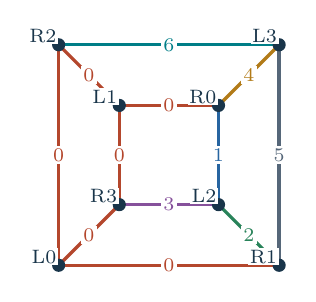
\begin{tikzpicture}[scale=1.4,every node/.style={font=\scriptsize}]
\coordinate (v0) at (0,0);
\coordinate (v1) at (0.55,1.45);
\coordinate (v2) at (1.45,0.55);
\coordinate (v3) at (2,2);
\coordinate (v4) at (1.45,1.45);
\coordinate (v5) at (2,0);
\coordinate (v6) at (0,2);
\coordinate (v7) at (0.55,0.55);
\draw[line width=1.2pt,draw=c0] (v0) -- node[fill=white,inner sep=1pt,text=c0] {0} (v5);
\draw[line width=1.2pt,draw=c0] (v0) -- node[fill=white,inner sep=1pt,text=c0] {0} (v6);
\draw[line width=1.2pt,draw=c0] (v0) -- node[fill=white,inner sep=1pt,text=c0] {0} (v7);
\draw[line width=1.2pt,draw=c0] (v1) -- node[fill=white,inner sep=1pt,text=c0] {0} (v4);
\draw[line width=1.2pt,draw=c0] (v1) -- node[fill=white,inner sep=1pt,text=c0] {0} (v6);
\draw[line width=1.2pt,draw=c0] (v1) -- node[fill=white,inner sep=1pt,text=c0] {0} (v7);
\draw[line width=1.2pt,draw=c1] (v2) -- node[fill=white,inner sep=1pt,text=c1] {1} (v4);
\draw[line width=1.2pt,draw=c2] (v2) -- node[fill=white,inner sep=1pt,text=c2] {2} (v5);
\draw[line width=1.2pt,draw=c3] (v2) -- node[fill=white,inner sep=1pt,text=c3] {3} (v7);
\draw[line width=1.2pt,draw=c4] (v3) -- node[fill=white,inner sep=1pt,text=c4] {4} (v4);
\draw[line width=1.2pt,draw=c5] (v3) -- node[fill=white,inner sep=1pt,text=c5] {5} (v5);
\draw[line width=1.2pt,draw=c6] (v3) -- node[fill=white,inner sep=1pt,text=c6] {6} (v6);
\fill[ink] (v0) circle (1.7pt);
\node[above left,fill=white,inner sep=0.6pt,text=ink] at (v0) {L0};
\fill[ink] (v1) circle (1.7pt);
\node[above left,fill=white,inner sep=0.6pt,text=ink] at (v1) {L1};
\fill[ink] (v2) circle (1.7pt);
\node[above left,fill=white,inner sep=0.6pt,text=ink] at (v2) {L2};
\fill[ink] (v3) circle (1.7pt);
\node[above left,fill=white,inner sep=0.6pt,text=ink] at (v3) {L3};
\fill[ink] (v4) circle (1.7pt);
\node[above left,fill=white,inner sep=0.6pt,text=ink] at (v4) {R0};
\fill[ink] (v5) circle (1.7pt);
\node[above left,fill=white,inner sep=0.6pt,text=ink] at (v5) {R1};
\fill[ink] (v6) circle (1.7pt);
\node[above left,fill=white,inner sep=0.6pt,text=ink] at (v6) {R2};
\fill[ink] (v7) circle (1.7pt);
\node[above left,fill=white,inner sep=0.6pt,text=ink] at (v7) {R3};
\end{tikzpicture}\par{\scriptsize Sizes: $6,1,1,1,1,1,1$}\end{minipage}
\hfill
\begin{minipage}[t]{0.32\linewidth}\centering
\textbf{Class 2}\quad {\small $|O|=4$, $|S|=12$}\par\smallskip
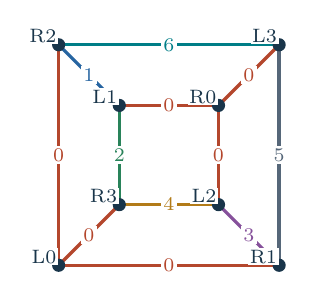
\begin{tikzpicture}[scale=1.4,every node/.style={font=\scriptsize}]
\coordinate (v0) at (0,0);
\coordinate (v1) at (0.55,1.45);
\coordinate (v2) at (1.45,0.55);
\coordinate (v3) at (2,2);
\coordinate (v4) at (1.45,1.45);
\coordinate (v5) at (2,0);
\coordinate (v6) at (0,2);
\coordinate (v7) at (0.55,0.55);
\draw[line width=1.2pt,draw=c0] (v0) -- node[fill=white,inner sep=1pt,text=c0] {0} (v5);
\draw[line width=1.2pt,draw=c0] (v0) -- node[fill=white,inner sep=1pt,text=c0] {0} (v6);
\draw[line width=1.2pt,draw=c0] (v0) -- node[fill=white,inner sep=1pt,text=c0] {0} (v7);
\draw[line width=1.2pt,draw=c0] (v1) -- node[fill=white,inner sep=1pt,text=c0] {0} (v4);
\draw[line width=1.2pt,draw=c1] (v1) -- node[fill=white,inner sep=1pt,text=c1] {1} (v6);
\draw[line width=1.2pt,draw=c2] (v1) -- node[fill=white,inner sep=1pt,text=c2] {2} (v7);
\draw[line width=1.2pt,draw=c0] (v2) -- node[fill=white,inner sep=1pt,text=c0] {0} (v4);
\draw[line width=1.2pt,draw=c3] (v2) -- node[fill=white,inner sep=1pt,text=c3] {3} (v5);
\draw[line width=1.2pt,draw=c4] (v2) -- node[fill=white,inner sep=1pt,text=c4] {4} (v7);
\draw[line width=1.2pt,draw=c0] (v3) -- node[fill=white,inner sep=1pt,text=c0] {0} (v4);
\draw[line width=1.2pt,draw=c5] (v3) -- node[fill=white,inner sep=1pt,text=c5] {5} (v5);
\draw[line width=1.2pt,draw=c6] (v3) -- node[fill=white,inner sep=1pt,text=c6] {6} (v6);
\fill[ink] (v0) circle (1.7pt);
\node[above left,fill=white,inner sep=0.6pt,text=ink] at (v0) {L0};
\fill[ink] (v1) circle (1.7pt);
\node[above left,fill=white,inner sep=0.6pt,text=ink] at (v1) {L1};
\fill[ink] (v2) circle (1.7pt);
\node[above left,fill=white,inner sep=0.6pt,text=ink] at (v2) {L2};
\fill[ink] (v3) circle (1.7pt);
\node[above left,fill=white,inner sep=0.6pt,text=ink] at (v3) {L3};
\fill[ink] (v4) circle (1.7pt);
\node[above left,fill=white,inner sep=0.6pt,text=ink] at (v4) {R0};
\fill[ink] (v5) circle (1.7pt);
\node[above left,fill=white,inner sep=0.6pt,text=ink] at (v5) {R1};
\fill[ink] (v6) circle (1.7pt);
\node[above left,fill=white,inner sep=0.6pt,text=ink] at (v6) {R2};
\fill[ink] (v7) circle (1.7pt);
\node[above left,fill=white,inner sep=0.6pt,text=ink] at (v7) {R3};
\end{tikzpicture}\par{\scriptsize Sizes: $6,1,1,1,1,1,1$}\end{minipage}
\hfill
\begin{minipage}[t]{0.32\linewidth}\centering
\textbf{Class 3}\quad {\small $|O|=4$, $|S|=12$}\par\smallskip
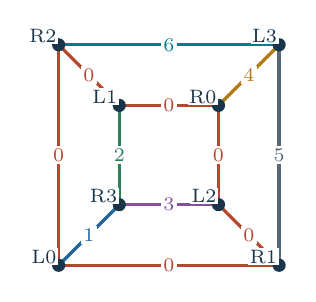
\begin{tikzpicture}[scale=1.4,every node/.style={font=\scriptsize}]
\coordinate (v0) at (0,0);
\coordinate (v1) at (0.55,1.45);
\coordinate (v2) at (1.45,0.55);
\coordinate (v3) at (2,2);
\coordinate (v4) at (1.45,1.45);
\coordinate (v5) at (2,0);
\coordinate (v6) at (0,2);
\coordinate (v7) at (0.55,0.55);
\draw[line width=1.2pt,draw=c0] (v0) -- node[fill=white,inner sep=1pt,text=c0] {0} (v5);
\draw[line width=1.2pt,draw=c0] (v0) -- node[fill=white,inner sep=1pt,text=c0] {0} (v6);
\draw[line width=1.2pt,draw=c1] (v0) -- node[fill=white,inner sep=1pt,text=c1] {1} (v7);
\draw[line width=1.2pt,draw=c0] (v1) -- node[fill=white,inner sep=1pt,text=c0] {0} (v4);
\draw[line width=1.2pt,draw=c0] (v1) -- node[fill=white,inner sep=1pt,text=c0] {0} (v6);
\draw[line width=1.2pt,draw=c2] (v1) -- node[fill=white,inner sep=1pt,text=c2] {2} (v7);
\draw[line width=1.2pt,draw=c0] (v2) -- node[fill=white,inner sep=1pt,text=c0] {0} (v4);
\draw[line width=1.2pt,draw=c0] (v2) -- node[fill=white,inner sep=1pt,text=c0] {0} (v5);
\draw[line width=1.2pt,draw=c3] (v2) -- node[fill=white,inner sep=1pt,text=c3] {3} (v7);
\draw[line width=1.2pt,draw=c4] (v3) -- node[fill=white,inner sep=1pt,text=c4] {4} (v4);
\draw[line width=1.2pt,draw=c5] (v3) -- node[fill=white,inner sep=1pt,text=c5] {5} (v5);
\draw[line width=1.2pt,draw=c6] (v3) -- node[fill=white,inner sep=1pt,text=c6] {6} (v6);
\fill[ink] (v0) circle (1.7pt);
\node[above left,fill=white,inner sep=0.6pt,text=ink] at (v0) {L0};
\fill[ink] (v1) circle (1.7pt);
\node[above left,fill=white,inner sep=0.6pt,text=ink] at (v1) {L1};
\fill[ink] (v2) circle (1.7pt);
\node[above left,fill=white,inner sep=0.6pt,text=ink] at (v2) {L2};
\fill[ink] (v3) circle (1.7pt);
\node[above left,fill=white,inner sep=0.6pt,text=ink] at (v3) {L3};
\fill[ink] (v4) circle (1.7pt);
\node[above left,fill=white,inner sep=0.6pt,text=ink] at (v4) {R0};
\fill[ink] (v5) circle (1.7pt);
\node[above left,fill=white,inner sep=0.6pt,text=ink] at (v5) {R1};
\fill[ink] (v6) circle (1.7pt);
\node[above left,fill=white,inner sep=0.6pt,text=ink] at (v6) {R2};
\fill[ink] (v7) circle (1.7pt);
\node[above left,fill=white,inner sep=0.6pt,text=ink] at (v7) {R3};
\end{tikzpicture}\par{\scriptsize Sizes: $6,1,1,1,1,1,1$}\end{minipage}
\par\vspace{1.1em}
\begin{minipage}[t]{0.32\linewidth}\centering
\textbf{Class 4}\quad {\small $|O|=48$, $|S|=1$}\par\smallskip
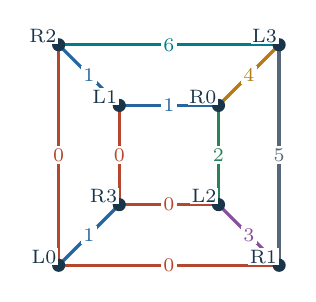
\begin{tikzpicture}[scale=1.4,every node/.style={font=\scriptsize}]
\coordinate (v0) at (0,0);
\coordinate (v1) at (0.55,1.45);
\coordinate (v2) at (1.45,0.55);
\coordinate (v3) at (2,2);
\coordinate (v4) at (1.45,1.45);
\coordinate (v5) at (2,0);
\coordinate (v6) at (0,2);
\coordinate (v7) at (0.55,0.55);
\draw[line width=1.2pt,draw=c0] (v0) -- node[fill=white,inner sep=1pt,text=c0] {0} (v5);
\draw[line width=1.2pt,draw=c0] (v0) -- node[fill=white,inner sep=1pt,text=c0] {0} (v6);
\draw[line width=1.2pt,draw=c1] (v0) -- node[fill=white,inner sep=1pt,text=c1] {1} (v7);
\draw[line width=1.2pt,draw=c1] (v1) -- node[fill=white,inner sep=1pt,text=c1] {1} (v4);
\draw[line width=1.2pt,draw=c1] (v1) -- node[fill=white,inner sep=1pt,text=c1] {1} (v6);
\draw[line width=1.2pt,draw=c0] (v1) -- node[fill=white,inner sep=1pt,text=c0] {0} (v7);
\draw[line width=1.2pt,draw=c2] (v2) -- node[fill=white,inner sep=1pt,text=c2] {2} (v4);
\draw[line width=1.2pt,draw=c3] (v2) -- node[fill=white,inner sep=1pt,text=c3] {3} (v5);
\draw[line width=1.2pt,draw=c0] (v2) -- node[fill=white,inner sep=1pt,text=c0] {0} (v7);
\draw[line width=1.2pt,draw=c4] (v3) -- node[fill=white,inner sep=1pt,text=c4] {4} (v4);
\draw[line width=1.2pt,draw=c5] (v3) -- node[fill=white,inner sep=1pt,text=c5] {5} (v5);
\draw[line width=1.2pt,draw=c6] (v3) -- node[fill=white,inner sep=1pt,text=c6] {6} (v6);
\fill[ink] (v0) circle (1.7pt);
\node[above left,fill=white,inner sep=0.6pt,text=ink] at (v0) {L0};
\fill[ink] (v1) circle (1.7pt);
\node[above left,fill=white,inner sep=0.6pt,text=ink] at (v1) {L1};
\fill[ink] (v2) circle (1.7pt);
\node[above left,fill=white,inner sep=0.6pt,text=ink] at (v2) {L2};
\fill[ink] (v3) circle (1.7pt);
\node[above left,fill=white,inner sep=0.6pt,text=ink] at (v3) {L3};
\fill[ink] (v4) circle (1.7pt);
\node[above left,fill=white,inner sep=0.6pt,text=ink] at (v4) {R0};
\fill[ink] (v5) circle (1.7pt);
\node[above left,fill=white,inner sep=0.6pt,text=ink] at (v5) {R1};
\fill[ink] (v6) circle (1.7pt);
\node[above left,fill=white,inner sep=0.6pt,text=ink] at (v6) {R2};
\fill[ink] (v7) circle (1.7pt);
\node[above left,fill=white,inner sep=0.6pt,text=ink] at (v7) {R3};
\end{tikzpicture}\par{\scriptsize Sizes: $4,3,1,1,1,1,1$}\end{minipage}
\hfill
\begin{minipage}[t]{0.32\linewidth}\centering
\textbf{Class 5}\quad {\small $|O|=12$, $|S|=4$}\par\smallskip
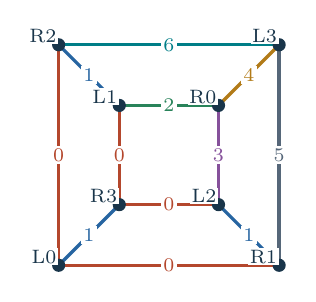
\begin{tikzpicture}[scale=1.4,every node/.style={font=\scriptsize}]
\coordinate (v0) at (0,0);
\coordinate (v1) at (0.55,1.45);
\coordinate (v2) at (1.45,0.55);
\coordinate (v3) at (2,2);
\coordinate (v4) at (1.45,1.45);
\coordinate (v5) at (2,0);
\coordinate (v6) at (0,2);
\coordinate (v7) at (0.55,0.55);
\draw[line width=1.2pt,draw=c0] (v0) -- node[fill=white,inner sep=1pt,text=c0] {0} (v5);
\draw[line width=1.2pt,draw=c0] (v0) -- node[fill=white,inner sep=1pt,text=c0] {0} (v6);
\draw[line width=1.2pt,draw=c1] (v0) -- node[fill=white,inner sep=1pt,text=c1] {1} (v7);
\draw[line width=1.2pt,draw=c2] (v1) -- node[fill=white,inner sep=1pt,text=c2] {2} (v4);
\draw[line width=1.2pt,draw=c1] (v1) -- node[fill=white,inner sep=1pt,text=c1] {1} (v6);
\draw[line width=1.2pt,draw=c0] (v1) -- node[fill=white,inner sep=1pt,text=c0] {0} (v7);
\draw[line width=1.2pt,draw=c3] (v2) -- node[fill=white,inner sep=1pt,text=c3] {3} (v4);
\draw[line width=1.2pt,draw=c1] (v2) -- node[fill=white,inner sep=1pt,text=c1] {1} (v5);
\draw[line width=1.2pt,draw=c0] (v2) -- node[fill=white,inner sep=1pt,text=c0] {0} (v7);
\draw[line width=1.2pt,draw=c4] (v3) -- node[fill=white,inner sep=1pt,text=c4] {4} (v4);
\draw[line width=1.2pt,draw=c5] (v3) -- node[fill=white,inner sep=1pt,text=c5] {5} (v5);
\draw[line width=1.2pt,draw=c6] (v3) -- node[fill=white,inner sep=1pt,text=c6] {6} (v6);
\fill[ink] (v0) circle (1.7pt);
\node[above left,fill=white,inner sep=0.6pt,text=ink] at (v0) {L0};
\fill[ink] (v1) circle (1.7pt);
\node[above left,fill=white,inner sep=0.6pt,text=ink] at (v1) {L1};
\fill[ink] (v2) circle (1.7pt);
\node[above left,fill=white,inner sep=0.6pt,text=ink] at (v2) {L2};
\fill[ink] (v3) circle (1.7pt);
\node[above left,fill=white,inner sep=0.6pt,text=ink] at (v3) {L3};
\fill[ink] (v4) circle (1.7pt);
\node[above left,fill=white,inner sep=0.6pt,text=ink] at (v4) {R0};
\fill[ink] (v5) circle (1.7pt);
\node[above left,fill=white,inner sep=0.6pt,text=ink] at (v5) {R1};
\fill[ink] (v6) circle (1.7pt);
\node[above left,fill=white,inner sep=0.6pt,text=ink] at (v6) {R2};
\fill[ink] (v7) circle (1.7pt);
\node[above left,fill=white,inner sep=0.6pt,text=ink] at (v7) {R3};
\end{tikzpicture}\par{\scriptsize Sizes: $4,3,1,1,1,1,1$}\end{minipage}
\hfill
\begin{minipage}[t]{0.32\linewidth}\centering
\textbf{Class 6}\quad {\small $|O|=48$, $|S|=1$}\par\smallskip
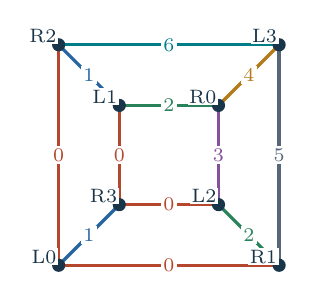
\begin{tikzpicture}[scale=1.4,every node/.style={font=\scriptsize}]
\coordinate (v0) at (0,0);
\coordinate (v1) at (0.55,1.45);
\coordinate (v2) at (1.45,0.55);
\coordinate (v3) at (2,2);
\coordinate (v4) at (1.45,1.45);
\coordinate (v5) at (2,0);
\coordinate (v6) at (0,2);
\coordinate (v7) at (0.55,0.55);
\draw[line width=1.2pt,draw=c0] (v0) -- node[fill=white,inner sep=1pt,text=c0] {0} (v5);
\draw[line width=1.2pt,draw=c0] (v0) -- node[fill=white,inner sep=1pt,text=c0] {0} (v6);
\draw[line width=1.2pt,draw=c1] (v0) -- node[fill=white,inner sep=1pt,text=c1] {1} (v7);
\draw[line width=1.2pt,draw=c2] (v1) -- node[fill=white,inner sep=1pt,text=c2] {2} (v4);
\draw[line width=1.2pt,draw=c1] (v1) -- node[fill=white,inner sep=1pt,text=c1] {1} (v6);
\draw[line width=1.2pt,draw=c0] (v1) -- node[fill=white,inner sep=1pt,text=c0] {0} (v7);
\draw[line width=1.2pt,draw=c3] (v2) -- node[fill=white,inner sep=1pt,text=c3] {3} (v4);
\draw[line width=1.2pt,draw=c2] (v2) -- node[fill=white,inner sep=1pt,text=c2] {2} (v5);
\draw[line width=1.2pt,draw=c0] (v2) -- node[fill=white,inner sep=1pt,text=c0] {0} (v7);
\draw[line width=1.2pt,draw=c4] (v3) -- node[fill=white,inner sep=1pt,text=c4] {4} (v4);
\draw[line width=1.2pt,draw=c5] (v3) -- node[fill=white,inner sep=1pt,text=c5] {5} (v5);
\draw[line width=1.2pt,draw=c6] (v3) -- node[fill=white,inner sep=1pt,text=c6] {6} (v6);
\fill[ink] (v0) circle (1.7pt);
\node[above left,fill=white,inner sep=0.6pt,text=ink] at (v0) {L0};
\fill[ink] (v1) circle (1.7pt);
\node[above left,fill=white,inner sep=0.6pt,text=ink] at (v1) {L1};
\fill[ink] (v2) circle (1.7pt);
\node[above left,fill=white,inner sep=0.6pt,text=ink] at (v2) {L2};
\fill[ink] (v3) circle (1.7pt);
\node[above left,fill=white,inner sep=0.6pt,text=ink] at (v3) {L3};
\fill[ink] (v4) circle (1.7pt);
\node[above left,fill=white,inner sep=0.6pt,text=ink] at (v4) {R0};
\fill[ink] (v5) circle (1.7pt);
\node[above left,fill=white,inner sep=0.6pt,text=ink] at (v5) {R1};
\fill[ink] (v6) circle (1.7pt);
\node[above left,fill=white,inner sep=0.6pt,text=ink] at (v6) {R2};
\fill[ink] (v7) circle (1.7pt);
\node[above left,fill=white,inner sep=0.6pt,text=ink] at (v7) {R3};
\end{tikzpicture}\par{\scriptsize Sizes: $4,2,2,1,1,1,1$}\end{minipage}
\par\vspace{1.1em}
\begin{minipage}[t]{0.32\linewidth}\centering
\textbf{Class 7}\quad {\small $|O|=24$, $|S|=2$}\par\smallskip
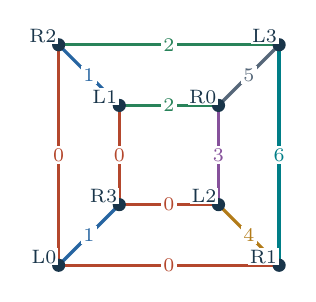
\begin{tikzpicture}[scale=1.4,every node/.style={font=\scriptsize}]
\coordinate (v0) at (0,0);
\coordinate (v1) at (0.55,1.45);
\coordinate (v2) at (1.45,0.55);
\coordinate (v3) at (2,2);
\coordinate (v4) at (1.45,1.45);
\coordinate (v5) at (2,0);
\coordinate (v6) at (0,2);
\coordinate (v7) at (0.55,0.55);
\draw[line width=1.2pt,draw=c0] (v0) -- node[fill=white,inner sep=1pt,text=c0] {0} (v5);
\draw[line width=1.2pt,draw=c0] (v0) -- node[fill=white,inner sep=1pt,text=c0] {0} (v6);
\draw[line width=1.2pt,draw=c1] (v0) -- node[fill=white,inner sep=1pt,text=c1] {1} (v7);
\draw[line width=1.2pt,draw=c2] (v1) -- node[fill=white,inner sep=1pt,text=c2] {2} (v4);
\draw[line width=1.2pt,draw=c1] (v1) -- node[fill=white,inner sep=1pt,text=c1] {1} (v6);
\draw[line width=1.2pt,draw=c0] (v1) -- node[fill=white,inner sep=1pt,text=c0] {0} (v7);
\draw[line width=1.2pt,draw=c3] (v2) -- node[fill=white,inner sep=1pt,text=c3] {3} (v4);
\draw[line width=1.2pt,draw=c4] (v2) -- node[fill=white,inner sep=1pt,text=c4] {4} (v5);
\draw[line width=1.2pt,draw=c0] (v2) -- node[fill=white,inner sep=1pt,text=c0] {0} (v7);
\draw[line width=1.2pt,draw=c5] (v3) -- node[fill=white,inner sep=1pt,text=c5] {5} (v4);
\draw[line width=1.2pt,draw=c6] (v3) -- node[fill=white,inner sep=1pt,text=c6] {6} (v5);
\draw[line width=1.2pt,draw=c2] (v3) -- node[fill=white,inner sep=1pt,text=c2] {2} (v6);
\fill[ink] (v0) circle (1.7pt);
\node[above left,fill=white,inner sep=0.6pt,text=ink] at (v0) {L0};
\fill[ink] (v1) circle (1.7pt);
\node[above left,fill=white,inner sep=0.6pt,text=ink] at (v1) {L1};
\fill[ink] (v2) circle (1.7pt);
\node[above left,fill=white,inner sep=0.6pt,text=ink] at (v2) {L2};
\fill[ink] (v3) circle (1.7pt);
\node[above left,fill=white,inner sep=0.6pt,text=ink] at (v3) {L3};
\fill[ink] (v4) circle (1.7pt);
\node[above left,fill=white,inner sep=0.6pt,text=ink] at (v4) {R0};
\fill[ink] (v5) circle (1.7pt);
\node[above left,fill=white,inner sep=0.6pt,text=ink] at (v5) {R1};
\fill[ink] (v6) circle (1.7pt);
\node[above left,fill=white,inner sep=0.6pt,text=ink] at (v6) {R2};
\fill[ink] (v7) circle (1.7pt);
\node[above left,fill=white,inner sep=0.6pt,text=ink] at (v7) {R3};
\end{tikzpicture}\par{\scriptsize Sizes: $4,2,2,1,1,1,1$}\end{minipage}
\hfill
\begin{minipage}[t]{0.32\linewidth}\centering
\textbf{Class 8}\quad {\small $|O|=6$, $|S|=8$}\par\smallskip
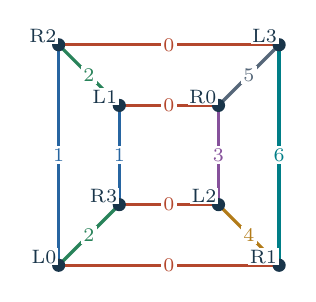
\begin{tikzpicture}[scale=1.4,every node/.style={font=\scriptsize}]
\coordinate (v0) at (0,0);
\coordinate (v1) at (0.55,1.45);
\coordinate (v2) at (1.45,0.55);
\coordinate (v3) at (2,2);
\coordinate (v4) at (1.45,1.45);
\coordinate (v5) at (2,0);
\coordinate (v6) at (0,2);
\coordinate (v7) at (0.55,0.55);
\draw[line width=1.2pt,draw=c0] (v0) -- node[fill=white,inner sep=1pt,text=c0] {0} (v5);
\draw[line width=1.2pt,draw=c1] (v0) -- node[fill=white,inner sep=1pt,text=c1] {1} (v6);
\draw[line width=1.2pt,draw=c2] (v0) -- node[fill=white,inner sep=1pt,text=c2] {2} (v7);
\draw[line width=1.2pt,draw=c0] (v1) -- node[fill=white,inner sep=1pt,text=c0] {0} (v4);
\draw[line width=1.2pt,draw=c2] (v1) -- node[fill=white,inner sep=1pt,text=c2] {2} (v6);
\draw[line width=1.2pt,draw=c1] (v1) -- node[fill=white,inner sep=1pt,text=c1] {1} (v7);
\draw[line width=1.2pt,draw=c3] (v2) -- node[fill=white,inner sep=1pt,text=c3] {3} (v4);
\draw[line width=1.2pt,draw=c4] (v2) -- node[fill=white,inner sep=1pt,text=c4] {4} (v5);
\draw[line width=1.2pt,draw=c0] (v2) -- node[fill=white,inner sep=1pt,text=c0] {0} (v7);
\draw[line width=1.2pt,draw=c5] (v3) -- node[fill=white,inner sep=1pt,text=c5] {5} (v4);
\draw[line width=1.2pt,draw=c6] (v3) -- node[fill=white,inner sep=1pt,text=c6] {6} (v5);
\draw[line width=1.2pt,draw=c0] (v3) -- node[fill=white,inner sep=1pt,text=c0] {0} (v6);
\fill[ink] (v0) circle (1.7pt);
\node[above left,fill=white,inner sep=0.6pt,text=ink] at (v0) {L0};
\fill[ink] (v1) circle (1.7pt);
\node[above left,fill=white,inner sep=0.6pt,text=ink] at (v1) {L1};
\fill[ink] (v2) circle (1.7pt);
\node[above left,fill=white,inner sep=0.6pt,text=ink] at (v2) {L2};
\fill[ink] (v3) circle (1.7pt);
\node[above left,fill=white,inner sep=0.6pt,text=ink] at (v3) {L3};
\fill[ink] (v4) circle (1.7pt);
\node[above left,fill=white,inner sep=0.6pt,text=ink] at (v4) {R0};
\fill[ink] (v5) circle (1.7pt);
\node[above left,fill=white,inner sep=0.6pt,text=ink] at (v5) {R1};
\fill[ink] (v6) circle (1.7pt);
\node[above left,fill=white,inner sep=0.6pt,text=ink] at (v6) {R2};
\fill[ink] (v7) circle (1.7pt);
\node[above left,fill=white,inner sep=0.6pt,text=ink] at (v7) {R3};
\end{tikzpicture}\par{\scriptsize Sizes: $4,2,2,1,1,1,1$}\end{minipage}
\hfill
\begin{minipage}[t]{0.32\linewidth}\centering
\textbf{Class 9}\quad {\small $|O|=16$, $|S|=3$}\par\smallskip
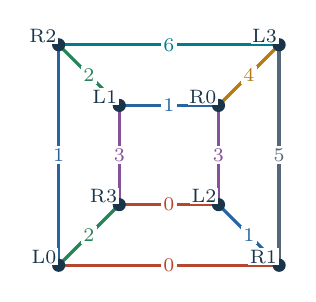
\begin{tikzpicture}[scale=1.4,every node/.style={font=\scriptsize}]
\coordinate (v0) at (0,0);
\coordinate (v1) at (0.55,1.45);
\coordinate (v2) at (1.45,0.55);
\coordinate (v3) at (2,2);
\coordinate (v4) at (1.45,1.45);
\coordinate (v5) at (2,0);
\coordinate (v6) at (0,2);
\coordinate (v7) at (0.55,0.55);
\draw[line width=1.2pt,draw=c0] (v0) -- node[fill=white,inner sep=1pt,text=c0] {0} (v5);
\draw[line width=1.2pt,draw=c1] (v0) -- node[fill=white,inner sep=1pt,text=c1] {1} (v6);
\draw[line width=1.2pt,draw=c2] (v0) -- node[fill=white,inner sep=1pt,text=c2] {2} (v7);
\draw[line width=1.2pt,draw=c1] (v1) -- node[fill=white,inner sep=1pt,text=c1] {1} (v4);
\draw[line width=1.2pt,draw=c2] (v1) -- node[fill=white,inner sep=1pt,text=c2] {2} (v6);
\draw[line width=1.2pt,draw=c3] (v1) -- node[fill=white,inner sep=1pt,text=c3] {3} (v7);
\draw[line width=1.2pt,draw=c3] (v2) -- node[fill=white,inner sep=1pt,text=c3] {3} (v4);
\draw[line width=1.2pt,draw=c1] (v2) -- node[fill=white,inner sep=1pt,text=c1] {1} (v5);
\draw[line width=1.2pt,draw=c0] (v2) -- node[fill=white,inner sep=1pt,text=c0] {0} (v7);
\draw[line width=1.2pt,draw=c4] (v3) -- node[fill=white,inner sep=1pt,text=c4] {4} (v4);
\draw[line width=1.2pt,draw=c5] (v3) -- node[fill=white,inner sep=1pt,text=c5] {5} (v5);
\draw[line width=1.2pt,draw=c6] (v3) -- node[fill=white,inner sep=1pt,text=c6] {6} (v6);
\fill[ink] (v0) circle (1.7pt);
\node[above left,fill=white,inner sep=0.6pt,text=ink] at (v0) {L0};
\fill[ink] (v1) circle (1.7pt);
\node[above left,fill=white,inner sep=0.6pt,text=ink] at (v1) {L1};
\fill[ink] (v2) circle (1.7pt);
\node[above left,fill=white,inner sep=0.6pt,text=ink] at (v2) {L2};
\fill[ink] (v3) circle (1.7pt);
\node[above left,fill=white,inner sep=0.6pt,text=ink] at (v3) {L3};
\fill[ink] (v4) circle (1.7pt);
\node[above left,fill=white,inner sep=0.6pt,text=ink] at (v4) {R0};
\fill[ink] (v5) circle (1.7pt);
\node[above left,fill=white,inner sep=0.6pt,text=ink] at (v5) {R1};
\fill[ink] (v6) circle (1.7pt);
\node[above left,fill=white,inner sep=0.6pt,text=ink] at (v6) {R2};
\fill[ink] (v7) circle (1.7pt);
\node[above left,fill=white,inner sep=0.6pt,text=ink] at (v7) {R3};
\end{tikzpicture}\par{\scriptsize Sizes: $3,2,2,2,1,1,1$}\end{minipage}
\par\vspace{1.1em}
\end{center}
The displayed labels determine the partitions exactly, including when two
edge colors are visually similar. Vertices are identified across panels by
their labels; equivalence in the table permits all 48 cube automorphisms.

\newpage
\section{Structure and verification}
The first three classes all have color-class sizes $(6,1,1,1,1,1,1)$.
They are nevertheless inequivalent: the sorted vertex-degree sequences of
their six-edge color classes are respectively
\[
 (3,3,2,2,1,1,0,0),\quad
 (3,3,1,1,1,1,1,1),\quad
 (2,2,2,2,2,2,0,0).
\]
The second consists of two disjoint three-edge stars; the third is a
six-cycle. All vertex degrees above are in the monochromatic subgraph,
with isolated vertices retained. Degree sequences are graph invariants, so
these three classes cannot be identified by a cube automorphism.

Other repeated size profiles also conceal differences. Among the nine perfect
matchings, class 4 always has color multiplicities $(2,1,1)$, whereas class 5
has one matching with multiplicities $(3,1)$. Classes 6, 7, and 8 have the
same block sizes, but their exceptional matching profiles are respectively
none, $(2,2)$, and $(4)$. Thus class 8 contains a monochromatic perfect
matching. These are properties of the recorded finite classes, not general
classification theorems for larger graphs.

The collision audit gives $(U,O)=(1,0)$ for 150 extremizers and $(U,O)=(0,1)$
for the other 24, exactly class 7. It checks the one-class bound on all
$2^{12}-1=4095$ nonempty edge subsets as a separate implementation check.

\subsection*{Coverage and checks}
Restricted-growth strings with exactly seven blocks are enumerated without
rainbow-prefix pruning. Their total is checked against the independent
recurrence, starting from $S(0,0)=1$ and zero outside the admissible range:
\[
 S(n,k)=kS(n-1,k)+S(n-1,k-1).
\]
Each candidate is tested against all
nine perfect matchings. Each orbit is formed explicitly, normalized by color
renaming, and removed from the remaining population. The computation checks
disjointness, closure in the avoiding population, and orbit--stabilizer counts.

Tests separately enumerate all $8!$ vertex bijections and retain exactly
the adjacency-preserving maps. Their edge actions equal the 48 constructed
actions. All four-edge subsets independently reconstruct the perfect
matchings. A direct equal-color-pair test validates every saved orbit member;
the earlier full search independently checks the proved maximum and the
population count. These are implementation checks, not external refereeing.

\subsection*{Reproduction and interpretation}
From the repository root, with Python 3.11 or later:
\begin{quote}\small\ttfamily
python -m experiments.classify\_cube\par
python -m unittest discover -s tests -v
\end{quote}
The full dataset in \texttt{results/data/cube\_classification.json} includes
all 174 members, the edge order, and the nine matching constraints. The SVG
atlas and this source are regenerated by
\texttt{python -m experiments.render\_cube\_atlas}.
The detailed project report records provenance and the limited literature
search. No assertion of originality or currently open status follows from
this computation. The diagrams illustrate the classification; they do not
replace its enumerative coverage argument.
\end{document}
